%%%%%%%%%%%%%%%%%%%%%%%%%%%%%%%%%%%%%%%%%%%%%%%%%%%%%%%%%%%%%%%%%%%%%%
%% Briefings in Bioinformatics, Problem Solving Protocol           %%
%% OUP authoring template (oup-authoring-template.cls, CTAN v1.5)    %%
%%                                                                   %%
%% Built by scripts/bib_build.py, which copies the figures, builds   %%
%% the Supplementary Data and compiles both. The BMC Bioinformatics  %%
%% version in submission/ is the audited source of every number;     %%
%% scripts/bib_build.py refuses to finish if a number quoted here is %%
%% absent from it.                                                   %%
%%%%%%%%%%%%%%%%%%%%%%%%%%%%%%%%%%%%%%%%%%%%%%%%%%%%%%%%%%%%%%%%%%%%%%

\documentclass[unnumsec,webpdf,contemporary,large,numbered]{oup-authoring-template}

\usepackage{booktabs}
\graphicspath{{figures/}}
% The biography column is narrow; TeX broke "Research" as "Resea-rch". Allow only valid breaks.
\hyphenation{Re-search Re-searchers}
\providecommand{\bibcommenthead}{}
\newcommand{\societylogo}{}

\begin{document}

\journaltitle{Briefings in Bioinformatics}
\DOI{DOI added during production}
\copyrightyear{2026}
\pubyear{2026}
\vol{00}
\issue{0}
\access{Advance Access Publication Date: Day Month Year}
\appnotes{Problem Solving Protocol}

\firstpage{1}

\title[Auditing cross-cohort feature-selection benchmarks]{Auditing cross-cohort feature-selection benchmarks: cohort composition and tissue-context-dependent confounding across kidney, liver and colon transcriptomes}

\author[1,$\ast$]{Dohun Kim}
\author[1]{Minho Bae}
\author[1]{Jinho Park}
\author[1]{Hayoung Lee}
\author[1]{Hyeokjin Lim}
\author[1]{Seonghee Lee}

\address[1]{\orgdiv{Autonomous Intelligence DX Research Section}, \orgname{Electronics and Telecommunications Research Institute}, \orgaddress{\state{Daejeon}, \country{Republic of Korea}}}

\corresp[$\ast$]{Corresponding author. \href{mailto:dohun@etri.re.kr}{dohun@etri.re.kr}}

\received{Date}{0}{Year}
\revised{Date}{0}{Year}
\accepted{Date}{0}{Year}

\abstract{We present a reusable audit protocol that quantifies the sensitivity of cross-cohort feature-selection benchmarks to cohort composition and control definition, and evaluates the benefits and costs of confounder correction. Over all 26 subsets of five harmonised diabetic kidney disease cohorts, the reproducibility difference between a stability selector and a co-expression hub criterion ranged from $-0.106$ to $+0.170$ across three-cohort subsets, while the mean external AUROC advantage for the evaluated stability-selector--hub comparison stayed positive: a single configuration does not settle which of them is more reproducible, and the instability was associated with how far cohorts agreed about effects; subsampling the colon cohorts to kidney sizes did not reproduce the kidney instability. The most reproducible signal was an immediate-early gene module that tracked biopsy versus surgical procurement in 8 of 9 kidney datasets rather than disease. Substituting a biopsy control retained only 14--56\% of the naive signal across seven diagnoses, and residualising on a handling score cut procurement-driven genes from 27\% to 5\% with no AUROC loss detected, on an interval too wide to establish that performance is preserved, whereas batch correction by cohort was inert; correction rewrote the candidate list, only 14 of 30 genes surviving. Applying the protocol to liver and colon, against predictions fixed before those data were read, located its limits: the module was lower in biopsy cases than surgical controls in 9 of 10 such cohorts across kidney and liver and was most prominent in the stability top 50 in kidney, but in colon, where both arms are biopsies, it rose with inflammation, so blanket residualisation on that score is not safe in every tissue. Two of three predictions failed in at least one tissue and are reported in full. The protocol is released as a reporting checklist with decision rules, the harmonised cohorts, the audit and the code.}

\keywords{feature selection; benchmarking; reproducibility; batch effects; pre-analytical variables; transcriptomics}

\boxedtext{Key Points}{
\begin{itemize}
\item We provide a reusable audit protocol for cross-cohort feature-selection benchmarks (patient-overlap and procurement audit, cohort-composition and control-definition sensitivity analyses, correction benchmark) and apply it against predictions fixed and hash-stamped before the data were read; the article reports no new biomarker.
\item A reproducibility comparison between feature-selection methods on public cohorts can change sign with the choice of cohorts, so it should be reported as an interval over all admissible cohort subsets and separately from predictive performance.
\item When every cohort shares a procurement asymmetry between cases and controls, the pre-analytical confounder becomes the most reproducible signal; in kidney an immediate-early module separated biopsy from surgical tissue in 8 of 9 datasets.
\item Where clinically defensible and available, a control obtained by the same procedure is the design alternative to prefer; residualising on a handling score worked in kidney but is tissue-conditional, because the module also rises with inflammation.
\item In a test against predictions fixed and hash-stamped in advance, verdict instability recurred in liver, whose cohorts disagree about effects, but not in colon, whose cohorts agree, and the confounder was most prominent among the most reproducible genes where every cohort shared that asymmetry.
\end{itemize}}

\maketitle

%%=============================================================%%
\section{Introduction}\label{sec:intro}
%%=============================================================%%

Transcriptomic biomarker discovery has converged on a common recipe: assemble public case/control
cohorts, select features that behave consistently across them, and report the signature with a
classification performance figure. Consistency across independent cohorts is expected to filter
dataset-specific noise, and a methods literature has grown around the idea, from multi-cohort
meta-analysis \cite{haynes2017} to stability selection \cite{meinshausen2010}. The pitfalls of
classifiers derived from high-dimensional expression data \cite{simon2003,whalen2022,diazuriarte2022}
and the impact of batch structure \cite{leek2010} are well catalogued.

Two assumptions underlie the recipe: that a feature reproducible across cohorts more likely
reflects disease biology, and that a benchmark comparing selection methods on a set of public
cohorts measures the methods rather than the cohorts. That a method comparison depends on how it
was set up is established \cite{boulesteix2013,jelizarow2010,ullmann2023,weber2019,mangul2019,norel2011,dehghani2021},
as is the instability of high-dimensional feature selection under resampling \cite{haury2011}.
What is missing for cross-cohort biomarker discovery is a quantification: varying the cohort
configuration is recommended practice, but reporting the resulting interval is not. A meta-analysis
of 28 filter feature-selection studies found that the number of datasets, baselines and new methods
alone explained 33\% of the variance in reported win rates \cite{ebiele2026}, and a recent
framework grades which layers of differential-expression evidence reproduce across fixed cohorts
\cite{angelakis2026}; neither varies which cohorts enter the comparison, and neither asks whether
the most reproducible signal is the disease.

We address this as a protocol problem. Diabetic kidney disease (DKD) is a suitable first setting
because its usable public cohorts are few enough to enumerate and numerous enough to resample.
The protocol places four checks around a conventional benchmark, each taking the
output of the last. \textit{Step 1, audit the input.} Cohorts go in; a table of patient overlap
across accessions and of the procurement route of each arm comes out, and a series that shares
patients with another is excluded. \textit{Step 2, vary the cohorts.} The benchmark is re-run on
every admissible subset of the surviving cohorts, and the difference between methods is reported
as a range with its sign changes rather than as one number. \textit{Step 3, vary the control.}
The case set is held fixed and the control group is replaced by one obtained the same way as the
cases, and the two rankings are compared. \textit{Step 4, benchmark the corrections.} Each
correction available for whatever confounder the first three steps expose is scored on how much
of it is removed and what that costs in external performance. Because findings in one disease cannot separate a
property of benchmarking from a property of its cohorts, we then fixed three predictions before
reading any liver or colon expression value, and report every verdict, including two failures.

Three contributions follow. First, we quantify how far a benchmark verdict depends on which
cohorts are in it, and give a procedure that reports the range of the method difference together
with predictive performance, so that one configuration is not generalised into a statement about
the methods. Second, we show that the most reproducible signal can be a procurement confounder
shared by every cohort, and compare what each available correction removes against what it
costs, down to the change in the candidate list itself. Third, applying the protocol to liver and
colon marks its boundary: the same score also rises with inflammation, so the correction that
works in kidney must not be applied blindly elsewhere. The protocol is released as a checklist
with decision rules (Table~\ref{tab:checklist}).

%%=============================================================%%
\section{Materials and methods}\label{sec:methods}
%%=============================================================%%

The four audit steps of the Introduction map onto the subsections below in order: step 1 onto
cohort assembly and audit, step 2 onto evaluation and cohort-composition sensitivity, and steps 3
and 4 onto the confounder score, corrections and control definition.
Table~\ref{tab:checklist} states the decision rule for each step.

\subsection{Cohort assembly and audit}\label{sec:cohorts}

Fifteen human DKD transcriptome series were retrieved from the Gene Expression Omnibus (GEO).
Patient identifiers recovered from sample titles revealed reuse invisible at the accession level,
and three series (GSE30122, GSE47183 and GSE99340) were excluded because the same patients would
otherwise sit on both sides of a leave-one-dataset-out split (Supplementary File~2). Residual
overlap that could not be removed is disclosed (Table~\ref{tab:overlap}): the two ERCB
compartments GSE104948 and GSE104954 share 55 subjects, and GSE30528 and GSE30529 share 9.

Five cohorts entered the discovery rotation and two served as compartment validation
(Table~\ref{tab:cohorts}) \cite{woroniecka2011,pan2018,grayson2018,fan2019,jin2026}. In every
cohort the cases are kidney biopsies and the controls are not; none of the five discovery
contrasts uses a biopsy-matched control group. Further datasets served specific tests: GSE175759
\cite{park2022}, GSE162830 \cite{eadon2021}, GSE142153 \cite{sur2021}, GSE1009
\cite{baelde2004}, GSE111154 \cite{sircar2018}, GSE20602 \cite{neusser2010}, GSE5406 (heart)
\cite{hannenhalli2006}, and the Kidney Precision Medicine Project (KPMP) single-nucleus atlas
\cite{elachkar2021,lake2023}, in which the 27 donors enrolled with chronic kidney disease (CKD) and a
recorded history of diabetes are treated as an operational DKD-proxy subset rather than a
registry-defined diagnosis.

\begin{table}[!t]
\caption{Subjects appearing in more than one retained kidney series}\label{tab:overlap}
\tabcolsep=3pt
\begin{tabular*}{\columnwidth}{@{\extracolsep\fill}llrrrr@{\extracolsep\fill}}
\toprule
Series A & Series B & Shared & DKD & Non-biopsy & Other \\
         &          &        & cases & controls & biopsy \\
\midrule
GSE104948 & GSE104954 & 55 & 5 & 1 & 49 \\
GSE30528 & GSE30529 & 9 & 5 & 4 & 0 \\
\botrule
\end{tabular*}
\begin{tablenotes}%
\item These are the same patients profiled in two compartments, not duplicate cohorts. Other biopsy are the non-diabetic kidney-disease biopsies used as the procurement-matched comparator; folds are not independent for them either.
\end{tablenotes}
\end{table}

\begin{table*}[!t]
\caption{Kidney transcriptome cohorts. Cases are biopsies in every cohort; controls are not}\label{tab:cohorts}
\tabcolsep=0pt
\begin{tabular*}{\textwidth}{@{\extracolsep\fill}llllrrl@{\extracolsep\fill}}
\toprule
Cohort & Role & Compartment & Platform & Cases & Controls & Control tissue \\
\midrule
GSE104948 & discovery & glomerulus & GPL22945/GPL24120 & 12 & 26 & donor, nephrectomy \\
GSE142025 & discovery & cortex & Illumina HiSeq4000 & 27 & 9 & nephrectomy \\
GSE294519 & discovery & tubulointerstitium & GPL24676 & 23 & 13 & nephrectomy \\
GSE30528 & discovery & glomerulus & GPL571 & 9 & 13 & nephrectomy \\
GSE96804 & discovery & glomerulus & GPL17586 & 41 & 20 & nephrectomy \\
GSE104954 & compartment & tubulointerstitium & GPL22945/GPL24120 & 17 & 26 & donor, nephrectomy \\
GSE30529 & compartment & tubulointerstitium & GPL571 & 10 & 12 & nephrectomy \\
\botrule
\end{tabular*}
\begin{tablenotes}%
\item Nephrectomy, tumour nephrectomy; donor, living kidney donor. All cohorts share the frozen 9,900-gene Entrez space. Compartment cohorts are the second compartment of donors already represented; they enter the procurement and comparator analyses but not the cohort-composition sweep, which requires independent cohorts.
\end{tablenotes}
\end{table*}

\subsection{Harmonisation and selection strategies}\label{sec:selectors}

Probes were mapped to Entrez Gene identifiers, multi-gene probes dropped and duplicates collapsed
by maximum mean, a rule fixed before analysis. The intersection over the four original discovery
cohorts is 9,900 genes; GSE294519 was mapped into this frozen space and covers 98.5\% of it. All
cross-cohort operations use per-cohort gene-wise $z$-scores, which use no label information.

Four strategies were compared on the same gene space and folds (Supplementary Note~S1 gives
definitions and equations). DEG\_meta combines per-cohort Welch $t$-statistics by weighted
Stouffer's method \cite{whitlock2005}. WGCNA\_hub ranks genes by intramodular connectivity in a
soft-thresholded correlation network \cite{langfelder2008}, as prior DKD work did
\cite{feng2021}; it is implemented directly and departs from canonical WGCNA in the respects
listed in Table~\ref{tab:comparator}, which Supplementary File~1 shows do not change any
conclusion. RBS is cross-cohort stability selection (robust biomarker score) combining importance,
within-cohort stability, cross-cohort reproducibility and perturbation robustness under a
sign-concordance gate; it stands in for the stability-selection family \cite{meinshausen2010} and
no novelty is claimed for it. RBS\_orth is RBS after the handling-score correction below.

\begin{table}[!t]
\caption{What the correlation-module comparator shares with canonical WGCNA}\label{tab:comparator}
\tabcolsep=2pt
\begin{tabular*}{\columnwidth}{@{\extracolsep\fill}p{17mm}p{24mm}p{24mm}l@{\extracolsep\fill}}
\toprule
Element & Canonical & Used here & Status \\
\midrule
Similarity & Pearson correlation & Pearson correlation & same \\
Adjacency & signed or unsigned power & unsigned power & restricted \\
Soft power & scale-free fit & fixed at $\beta = 6$ & differs \\
Modules & TOM, dynamic tree cut & clustering on correlation distance & differs \\
Hub score & kME & connectivity kIN & differs \\
Eigengene & first principal component & not computed & absent \\
\botrule
\end{tabular*}
\begin{tablenotes}%
\item We therefore call it a correlation-module comparator and do not claim it reproduces the reference package. A 32-variant grid in Supplementary File~1 tests every departure, and the package itself was run as a second comparator (Table~\ref{tab:selectors}).
\end{tablenotes}
\end{table}

\subsection{Evaluation and cohort-composition sensitivity}\label{sec:nulls}

Evaluation is leave-one-dataset-out (LODO): each strategy selects $K = 50$ genes on the training
cohorts, a plain $L_2$ logistic model is fitted on them, and the held-out cohort is scored.
Predictive performance is the mean external AUROC over folds; reproducibility is the mean pairwise
Jaccard index between the gene sets selected in different folds. The two are reported separately
throughout. Every AUROC is read against a random-signature null of 300 same-size gene sets and a
permuted-label null (Supplementary Note~S2). Method differences carry a paired patient-level
bootstrap of 200 replicates in which the whole evaluation, selection included, is repeated. The
headline benchmark uses the four cohorts fixed before analysis; the composition sweep adds
GSE294519 and repeats the complete benchmark on every subset of the five discovery cohorts of
size 2--5 (26 subsets), with 30 inner bootstrap replicates per cohort.

\subsection{Confounder score, corrections and control definition}\label{sec:corrections}

The immediate-early gene (IEG) module (\textit{FOS}, \textit{FOSB}, \textit{JUN}, \textit{JUNB},
\textit{EGR1}, \textit{ATF3}, \textit{DUSP1}, \textit{ZFP36}, \textit{NR4A1}, \textit{NR4A2},
\textit{BTG2}, \textit{EGR2}, \textit{EGR3}, \textit{IER2}, \textit{KLF2}, \textit{KLF4},
\textit{SOCS3}, \textit{DUSP2}, \textit{JUND}) gives a label-free per-sample handling score $h_i$,
its mean $z$-score. Residualisation removes that axis from every gene with a slope estimated
within class, because $h$ is nearly collinear with case status and a total slope would absorb the
disease difference:
\begin{equation}
\beta_j = \frac{\tilde{h}^{\top} \tilde{x}_j}{\tilde{h}^{\top} \tilde{h}} , \qquad
x_{ij}^{\text{corr}} = x_{ij} - (h_i - \bar{h}) \beta_j ,
\label{eq:resid}
\end{equation}
where tildes denote centring inside each class. Two analyses report the cost of this correction
and they are not the same run: the fold means use the headline stability configuration (inner
bootstrap $B = 150$), whereas the paired uncertainty analysis resamples patients within each
cohort and class, re-runs the whole leave-one-dataset-out evaluation in each of 200 replicates, and
uses a reduced inner bootstrap ($B = 30$) to make that affordable. The corrections compared were none, this
residualisation, RUVg with the module or with empirical controls \cite{risso2014},
surrogate-variable adjustment protecting the design \cite{leek2007}, and ComBat with cohort as
batch \cite{johnson2007}. Effect sizes are Hedges' $g$ \cite{hedges1981}. The specificity gate
keeps genes with $|g| \ge 0.5$ for DKD against the other biopsy diagnoses of ERCB.

The control-definition sensitivity analysis holds the case set fixed and replaces the non-biopsy
control by the remaining biopsy diagnoses of the same resource, then counts genes reaching
$|g| \ge 0.5$ under each definition and compares the top of the two rankings. It does not
separate clinical from pre-analytical causes; procurement is our reading of why the definitions
differ.

\subsection{Predictions fixed before the liver and colon data were read}\label{sec:xtmethods}

Instability of reproducibility verdicts is a statistical claim and should appear in any tissue; a
procurement confounder should become reproducible only where every cohort shares the same
asymmetry. Two tissues separate these. In liver with metabolic dysfunction-associated
steatohepatitis (MASH), procurement is asymmetric in some cohorts (needle biopsy cases, donor or
surgical controls) and matched in others; in ulcerative colitis (UC), both arms are endoscopic
biopsies in every cohort. Three predictions (P1--P3, stated in Results) were written after reading
only series- and sample-level metadata and before any expression value was downloaded; the file's
SHA-256 digest and time stamp were recorded, a second file stating post hoc analyses was hashed
before those analyses ran, and a pipeline stage verifies both digests on every run
(Supplementary File~7). The digests were recorded locally, so what they establish is that neither
file has changed since it was written, not an externally certified date: there is no third-party
registry entry. We therefore describe these as predictions stated and hash-fixed before the
analysis rather than as a registered protocol.

Cases were MASH against histologically normal liver and actively inflamed UC colon against
normal control colon, one sample per subject. Procurement was coded per arm from series text,
sample fields and source publications before any effect was computed. Five core cohorts per
tissue entered the composition sweep; remaining eligible cohorts entered only the per-cohort
module test. Patient reuse across same-platform series was audited on expression values: a sample
whose best partner in another series reached $r \ge 0.9999$ was called identical. The audit
excluded GSE59071 (116 samples identical to GSE75214) and GSE17470 (9 identical to GSE24807). Selection
used the genes shared by each tissue's core cohorts, 7,805 in liver (11 of the 19 module genes)
and 15,789 in colon (all 19), and the kidney code and parameters were reused unchanged. The
per-cohort effect $g_{\text{IEG}}$ is Hedges' $g$ of the handling score with a 1,000-resample
bootstrap interval. Post hoc, the effect was adjusted for a 13-gene inflammation score sharing no
gene with the module, cross-cohort effect concordance was defined as the median pairwise Spearman
correlation of gene-wise $g$, and colon cohorts were subsampled to kidney sizes in five
replicates (Supplementary Note~S10 gives the full cohort, audit and harmonisation rules).

\subsection{Implementation}\label{sec:implementation}

All analyses are implemented in Python with pinned versions and run from a single entry point
whose manuscript path is checked against a dependency closure of every declared output
(Supplementary Note~S9). Every resampling stage takes a fixed seed.

\textbf{Use of AI tools.} Claude Code (Anthropic) and ChatGPT (OpenAI) assisted with
code development and refactoring, proposals for control analyses, manuscript drafting and
revision, and figure preparation. Numerical results were computed from the cited datasets or
explicitly described simulations using the analysis code. Automated checks were used to assess
numerical consistency and provenance. The authors reviewed the code, analyses and manuscript and
take responsibility for the final content.
%% AUTHORS: journal-required AI disclosure. Confirm the last sentence (the scope of your own
%% review) and keep the cover-letter version identical.


%%=============================================================%%
\section{Results}\label{sec:results}
%%=============================================================%%

\subsection{Reproducibility verdicts depend on cohort composition}\label{sec:sensitivity}

Absolute AUROC was uninformative: random 50-gene sets reached 0.68--0.88 depending on the held-out
cohort, while permuted labels gave approximately 0.50, because the DKD programme is broadly
co-expressed (Supplementary Note~S2). The method comparison was no more stable. Across the ten
three-cohort subsets the paired difference RBS $-$ connectivity in cross-fold agreement spanned
$-0.106$ to $+0.170$ (Figure~\ref{fig:sensitivity}). A study using GSE96804 $+$ GSE142025 $+$
GSE294519 would report $+0.170$ in favour of stability selection, and one using GSE30528 $+$
GSE104948 $+$ GSE142025 would report $-0.106$ against it; both are legitimate DKD benchmarks.
RBS won on reproducibility in 9 of 10 three-cohort subsets and lost when all five cohorts were used.

External AUROC behaved differently. Its mean advantage was positive at every subset size and
grew with cohort count, to $+0.139$ at five cohorts. The paired bootstrap put that five-cohort
difference at $+0.129$ [$-0.002$, $+0.263$] ($p = 0.06$): the mean difference favoured
stability selection, but the interval included zero. The two metrics did not
even agree on the winner: excluding ties, the method first on reproducibility was first on
external AUROC in 11 of 24 subsets. A benchmark reporting one of these numbers is therefore not
reporting a weaker version of the other. Table~\ref{tab:checklist} lists what a benchmark on
public cohorts should report as a consequence.

The instability is not a property of one selector pair. Repeating the 26-subset sweep with each
of six further inner selectors of stability selection, against the same connectivity comparator,
reproduced it in every case (Table~\ref{tab:selectors}): the three-cohort reproducibility
difference changed sign under all seven selectors, in 1 to 5 of the 10 subsets, and with all five
cohorts the connectivity comparator won on reproducibility while stability selection won on
external AUROC under every selector. Random forest was the least stable, reversing in half of the
three-cohort subsets. What the seven share is the comparator and the cohorts, so the instability
belongs to the cohort set rather than to any selector, within the classical families tested.

The comparator side was checked the same way. Replacing the reimplementation by the WGCNA
package itself, run with its tutorial defaults on every fold (settings in the note to
Table~\ref{tab:selectors}), reproduced the reversal: the three-cohort difference spanned $-0.081$
to $+0.261$, and with all five cohorts the package won on reproducibility ($-0.133$) while
stability selection won on external AUROC ($+0.080$). The package was the weaker comparator on
both axes (mean Jaccard 0.064 and AUROC 0.711 over the 26 subsets, against 0.107 and 0.783 for
the reimplementation), so the reimplementation did not flatter stability selection.
\begin{figure*}[!t]
\centering
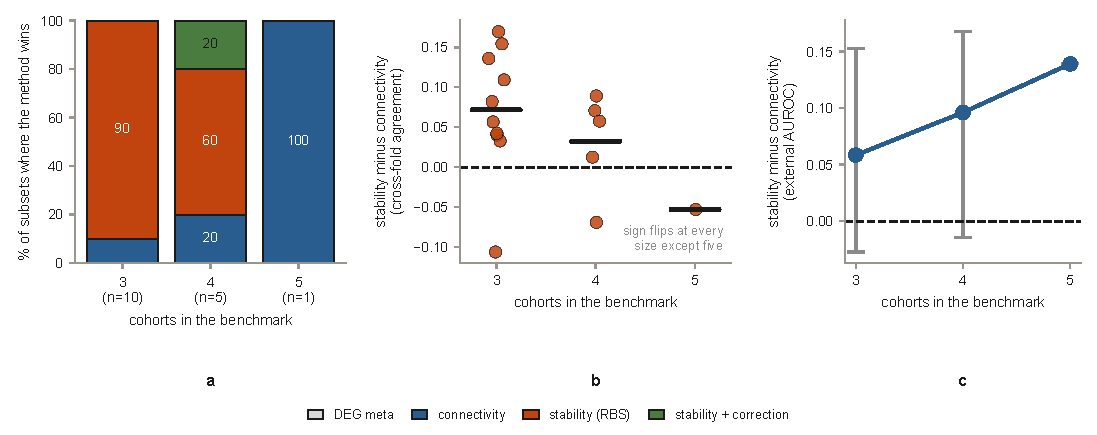
\includegraphics[width=\textwidth]{Fig1}
\caption{\textbf{The reproducibility verdict depends on which cohorts are in the benchmark; the mean predictive advantage stays positive.} The benchmark was repeated over all 26 subsets of the five discovery cohorts; panels show the 16 of size three or more. \textbf{a} Percentage of subsets in which each method wins on cross-fold reproducibility, ties excluded. \textbf{b} Stability selection minus the connectivity comparator in cross-fold agreement for every subset; the difference spans $-0.106$ to $+0.170$. \textbf{c} The same subsets scored by external AUROC, where the mean advantage is positive at every size ($+0.058$, $+0.096$, $+0.139$ for sizes three to five). Custom co-expression hub comparator; not the reference WGCNA implementation.}\label{fig:sensitivity}
\end{figure*}

\begin{table*}[!t]
\caption{The audit protocol as a checklist: what to report, why, and what to do when the check fails}\label{tab:checklist}
\tabcolsep=0pt
\begin{tabular*}{\textwidth}{@{\extracolsep\fill}>{\raggedright\arraybackslash}p{40mm}>{\raggedright\arraybackslash}p{44mm}>{\raggedright\arraybackslash}p{58mm}>{\raggedright\arraybackslash}p{28mm}@{\extracolsep\fill}}
\toprule
Report & Because & What to do when the check fails & Where applied \\
\midrule
A patient-overlap audit across accessions & reused patients make subsets and folds non-independent & exclude the duplicated series, and disclose the overlap that cannot be removed & Table~\ref{tab:overlap} \\
Procurement route of cases and of controls, per cohort & collinearity with diagnosis is a confounder no selector can remove & where no comparator shares the procurement route, hold the attribution open instead of naming a cause & Table~\ref{tab:cohorts}, Figure~\ref{fig:procurement} \\
Pre-analytical variables to the SPREC or BRISQ standard & they turn the inference into a measurable covariate & where unavailable, say so and keep procurement as an inference & unavailable in every cohort used \\
The method difference as a range over all admissible cohort subsets, and whether it changes sign & a single configuration is one draw from that range & report the range, not the single verdict; with too many cohorts to enumerate, draw a pre-specified sample of configurations and say how it was drawn & Figure~\ref{fig:sensitivity} \\
Cross-cohort concordance of gene-wise effects & low concordance is where sign changes appeared & treat a single-configuration ranking as local to those cohorts and withhold the general claim & Figures~\ref{fig:sensitivity}, \ref{fig:xtissue} \\
Winner frequency at a fixed subset size, ties excluded, with reproducibility and predictive performance side by side & with few folds ties inflate apparent wins, and the two metrics agreed on the winner in only 11 of 24 subsets & report both axes separately; do not let one stand in for the other & Figure~\ref{fig:sensitivity} \\
Every AUROC with its position in a random-signature null & random 50-gene sets reached 0.68--0.88 here & if the selected set does not clear its own null, report the margin rather than the absolute figure & Supplementary Note~S2 \\
A control obtained by the same procedure wherever one exists & it did more work here than any algorithm & where an alternative control exists, compare the rankings under both definitions; where none exists, state that this sensitivity cannot be assessed and treat the candidate order as conditional & Figures~\ref{fig:reordering}, \ref{fig:xtissue} \\
Whether the correction score also carries disease biology & the same module rose with inflammation in colon & assess how far the score overlaps the disease signal and report the selection with and without the correction; where the two cannot be separated on the available evidence, withhold blanket residualisation and prefer the design-based control & Figure~\ref{fig:xtissue} \\
\botrule
\end{tabular*}
\begin{tablenotes}%
\item The rows follow the four steps of the Methods in order: audit the input, vary the cohorts, vary the control, benchmark the corrections. The null-comparison row applies to every AUROC reported in any step. Each check was applied here; the last column says where the result appears.
\end{tablenotes}
\end{table*}

\begin{table*}[!t]
\caption{Verdict instability under each inner selector of stability selection}\label{tab:selectors}
\tabcolsep=0pt
\begin{tabular*}{\textwidth}{@{\extracolsep\fill}lrrrrrr@{\extracolsep\fill}}
\toprule
Inner selector & Cross-fold Jaccard, three cohorts & Neg. & External AUROC, three cohorts & Neg. & Jaccard, five & AUROC, five \\
\midrule
ReliefF (headline) & $-0.106$ to $+0.170$ & 1 & $-0.027$ to $+0.153$ & 2 & $-0.053$ & $+0.139$ \\
Univariate $F$     & $-0.111$ to $+0.150$ & 1 & $-0.098$ to $+0.150$ & 2 & $-0.063$ & $+0.101$ \\
LASSO              & $-0.127$ to $+0.119$ & 2 & $-0.112$ to $+0.146$ & 1 & $-0.090$ & $+0.078$ \\
Elastic net        & $-0.163$ to $+0.119$ & 2 & $-0.033$ to $+0.119$ & 1 & $-0.106$ & $+0.091$ \\
mRMR               & $-0.105$ to $+0.154$ & 1 & $-0.096$ to $+0.129$ & 2 & $-0.037$ & $+0.088$ \\
Random forest      & $-0.211$ to $+0.074$ & 5 & $-0.039$ to $+0.127$ & 3 & $-0.144$ & $+0.125$ \\
Boruta             & $-0.157$ to $+0.120$ & 2 & $-0.106$ to $+0.106$ & 3 & $-0.145$ & $+0.111$ \\
\midrule
\multicolumn{7}{l}{\textit{Comparator replaced by the WGCNA package (ReliefF inner selector)}} \\
WGCNA package      & $-0.081$ to $+0.261$ & 1 & $-0.007$ to $+0.283$ & 1 & $-0.133$ & $+0.080$ \\
\botrule
\end{tabular*}
\begin{tablenotes}%
\item Stability selection minus the connectivity comparator, the inner selector of stability selection varied; the comparator is unchanged. Ten three-cohort subsets per row; Neg., subsets in which the difference is negative. Five, the single five-cohort benchmark. Rows above the rule use the custom co-expression hub comparator, not the reference WGCNA implementation. The last row replaces the custom comparator by the WGCNA package run with its tutorial defaults on every fold (soft power by scale-free fit, 4--20 here; unsigned TOM; dynamic tree cut; module most correlated with the trait; hubs by $|$kME$|$).
\end{tablenotes}
\end{table*}

\subsection{The most reproducible signal tracks tissue procurement}\label{sec:procurement}

No DKD cohort we examined reports warm or cold ischaemia time, fixation or time to stabilisation,
so procurement route is read from sample annotations and its attribution to handling is an
inference. It rests on three observations. Across nine kidney datasets the IEG module was lower in
biopsy-procured than in nephrectomy- or donor-procured groups in eight (Figure~\ref{fig:procurement};
Spearman $\rho = -0.75$, $p < 0.001$); the exception, GSE162830, processed all 32 samples
identically and showed no effect ($-0.05$). In KPMP single-nucleus pseudobulk, DKD separated from
non-biopsy reference tissue ($p = 6.0\times10^{-76}$) but not from non-diabetic CKD, which is also
biopsied ($p = 0.21$; Supplementary Note~S3). And warm ischaemia induces exactly these transcripts
within minutes, including in kidney \cite{ma2012}, and drives transcriptome variation across human
tissues \cite{ferreira2018}. An independent comparison of reference tissue sources within KPMP has
since reported the same dependence \cite{menon2026}. In heart failure (GSE5406), where explanted
and donor hearts are handled similarly, the module separated explant from donor only weakly
($g = -0.23$).

Because this asymmetry is shared by every discovery contrast, the confounder is maximally
reproducible, and a criterion that rewards consistency ranks it first: uncorrected RBS placed 10
immediate-early genes in its top 50. The connectivity comparator placed none, but this exclusion
alone does not establish robustness. The
module's genes are strongly trait-correlated yet rank low by connectivity, because
intramodular connectivity sums adjacencies and rewards membership of large blocks: the median
block size is 19 for the immediate-early genes against 705 for the top 50 by connectivity. All 32
variants of the comparator placed no immediate-early gene in the top 50, and simulation shows the
advantage reverses when a confounder forms the larger block (Supplementary Note~S4). The WGCNA
package itself did not always exclude the module: across the 75 leave-one-dataset-out folds of the
cohort sweep, which evaluate 30 distinct training combinations, it placed at least one
immediate-early gene in its top 50 in 9 folds (3 distinct training combinations), up to 18 of 50,
and every such fold was one in which dynamic tree cut had produced a small trait module (61 to 199
genes, against a median of 588). The package ranks by $|$kME$|$ within the chosen module, so this
does not test the summed-connectivity account directly; the findings are consistent with
module-dependent exclusion rather than general robustness to confounding.

\begin{figure*}[!t]
\centering
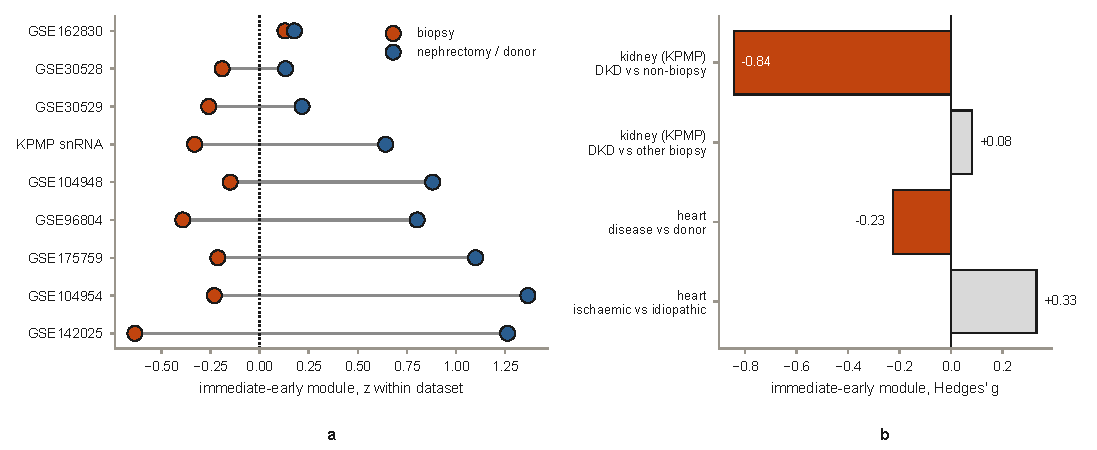
\includegraphics[width=\textwidth]{Fig2}
\caption{\textbf{The most reproducible signal tracks tissue procurement.} \textbf{a} The immediate-early module, $z$-scored within dataset, for every diagnosis group in nine kidney datasets. Biopsy-procured groups sit below nephrectomy- and donor-procured groups in eight of nine (Spearman $\rho = -0.75$, $p < 0.001$); GSE162830, the one identically processed design, is the exception. \textbf{b} The module as Hedges' $g$ for four contrasts. In KPMP, DKD against non-biopsy reference tissue gives $-0.84$ while DKD against other biopsies gives $+0.08$; in heart failure (GSE5406), disease against donor reaches only $-0.23$.}\label{fig:procurement}
\end{figure*}

\subsection{Which corrections work}\label{sec:whichcorrections}

ComBat with cohort as batch returned the same values as no correction in this implementation and
evaluation setting (Table~\ref{tab:corrections}, Figure~\ref{fig:corrections}). Cohort-level batch
adjustment alone cannot disentangle procurement from disease when the two are confounded within
cohorts. RUVg with empirical controls also
failed, so the control set rather than the framework does the work. Residualisation and
surrogate-variable adjustment reduced procurement-flagged genes from 27\% to 5--6\%. Table~\ref{tab:corrections}
reports identical fold-mean AUROCs to three decimal places. In a separate patient-stratified
paired bootstrap analysis with 200 replicates (Methods), the mean uncorrected
minus residualised difference was $+0.079$ (95\% percentile interval $-0.048$ to $+0.229$). This
exploratory uncertainty estimate does not establish performance preservation: a substantial loss
remains compatible with the interval, whose tails are imprecisely estimated. The
evaluation is not circular: the procurement flag derives from ERCB effect sizes, and correlation
with the handling score separates flagged from unflagged genes at AUC $= 0.480$. Across seven
inner selectors (Table~\ref{tab:sweep}), residualisation lowered the flagged fraction for every
one, from 17.0--35.5\% to 3.5--12.5\%, at an AUROC cost that ranged from a gain of 0.021 to a loss
of 0.114; a study adopting it should report that cost for its selector.

\begin{table}[!t]
\caption{Correction benchmark at $K = 50$}\label{tab:corrections}
\tabcolsep=1.5pt
\begin{tabular*}{\columnwidth}{@{\extracolsep\fill}lrrrrr@{\extracolsep\fill}}
\toprule
Correction & IEG & Flagged & Spec. & AUROC & Cross- \\
           & top 50 &     & pass  &       & fold \\
\midrule
None                      & 8.5 & 27\% & 33\% & 0.926 & 0.284 \\
ComBat (cohort)           & 8.5 & 27\% & 33\% & 0.926 & 0.284 \\
RUVg, empirical           & 7.5 & 28\% & 26\% & 0.924 & 0.154 \\
RUVg, module              & 0.8 & 18\% & 40\% & 0.905 & 0.215 \\
Surrogate variables       & 2.0 & 6\%  & 44\% & 0.915 & 0.251 \\
Residualise on $h$        & 1.0 & 5\%  & 40\% & 0.926 & 0.260 \\
\botrule
\end{tabular*}
\begin{tablenotes}%
\item IEG top 50 and the other columns are means over the leave-one-dataset-out folds, so the uncorrected count differs from the 10 of the single headline run. Flagged, procurement-flagged share of the top 50. Spec. pass, share clearing the DKD-versus-other-CKD gate, whose background pass rate is 8.3\% and permutation-based false-discovery estimate 16.7\%.
\end{tablenotes}
\end{table}

\begin{figure*}[!t]
\centering
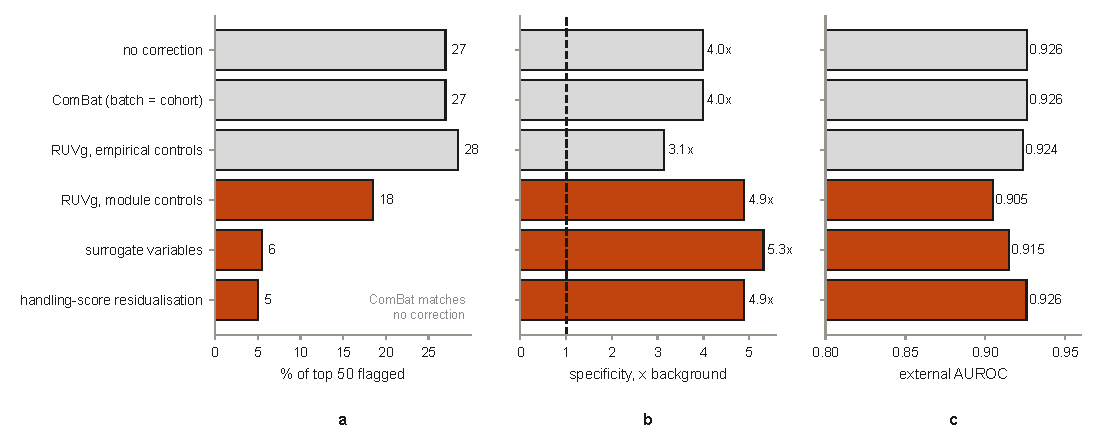
\includegraphics[width=\textwidth]{Fig3}
\caption{\textbf{What each correction removes, and what it costs.} \textbf{a} Percentage of the top 50 selected features flagged as procurement-driven. \textbf{b} Specificity pass-rate as fold-enrichment over the 8.3\% background rate at which a random gene passes the gate. \textbf{c} External AUROC. Handling-score residualisation and surrogate-variable analysis reduce procurement-driven features from 27\% to 5--6\%; residualisation does so at a fold-mean AUROC identical to no correction to three decimal places, surrogate-variable analysis at 0.915 against 0.926. The separate paired bootstrap estimate of the residualisation cost is uncertain and is given in the text. ComBat returned the same values as no correction in this evaluation setting; the confounder is within-cohort.}\label{fig:corrections}
\end{figure*}

\begin{table}[!t]
\caption{The handling-score correction under each inner selector ($K = 50$, $B = 40$)}\label{tab:sweep}
\tabcolsep=1.5pt
\begin{tabular*}{\columnwidth}{@{\extracolsep\fill}lrrrrr@{\extracolsep\fill}}
\toprule
Selector & \multicolumn{2}{c}{Flagged} & \multicolumn{2}{c}{AUROC} & Change \\
\cmidrule(lr){2-3}\cmidrule(lr){4-5}
 & before & after & before & after & in AUROC \\
\midrule
Univariate $F$ & 24.5\% & 6.0\%  & 0.921 & 0.807 & $-0.114$ \\
LASSO          & 33.0\% & 12.5\% & 0.956 & 0.879 & $-0.077$ \\
Elastic net    & 35.5\% & 3.5\%  & 0.909 & 0.857 & $-0.052$ \\
mRMR           & 28.0\% & 6.5\%  & 0.941 & 0.896 & $-0.046$ \\
ReliefF        & 29.5\% & 5.0\%  & 0.928 & 0.949 & $+0.021$ \\
Random forest  & 17.0\% & 7.5\%  & 0.895 & 0.815 & $-0.079$ \\
Boruta         & 22.0\% & 6.5\%  & 0.918 & 0.901 & $-0.017$ \\
\botrule
\end{tabular*}
\begin{tablenotes}%
\item Flagged, procurement-flagged share of the selected features; before and after the handling-score correction. Each row is a mean over the leave-one-dataset-out folds on the four headline cohorts. The correction lowers the flagged share for every selector; what it costs in AUROC does not follow the selector's uncorrected performance, so a study adopting it should report that cost for its own selector. The ReliefF row repeats Table~\ref{tab:corrections} at the lower $B$; the small differences are bootstrap resolution, not a change of method.
\end{tablenotes}
\end{table}

\subsection{The control-group problem is not specific to diabetic kidney disease}\label{sec:external}

The ERCB compartments contain eight biopsy diagnoses alongside the same non-biopsy controls, so
the control-definition analysis can ask inside one resource whether the effect belongs to DKD or to
the design. For each of seven diagnoses (thin membrane disease had too few cases), substituting
the other biopsy diagnoses for the non-biopsy control retained only 14--56\% of the naive median
effect size (Table~\ref{tab:ckdgen}); in IgA nephropathy the 3,800 genes reaching $|g| \ge 0.5$ fell to none
(Supplementary Note~S6). Diabetic nephropathy ranked fourth of seven. The substitution did not
merely shrink the signal; it rebuilt the top of the ranking (Figure~\ref{fig:reordering}). The 50
largest effects under the two definitions shared 1 gene in diabetic nephropathy, while rank
correlation over all 9,900 genes was 0.69, and the pipeline run with and without the handling-score
correction returned 30 candidates each, sharing only 14. Which genes a study nominates is
therefore set by how its control tissue was obtained as much as by the disease.

Two checks outside the discovery cohorts support the substitution. In GSE20602, which compares
nephrosclerosis glomeruli against tumour nephrectomy, the candidates moved further in the
diabetic contrast than in the nephrosclerosis one (median $|g_{\text{DKD}}| - |g_{\text{NSC}}|$ of
$+1.02$ against $-0.17$ for the remaining genes, Mann--Whitney $p = 5.1 \times 10^{-18}$). And the
comparator behaves the same way in a different molecular layer: replacing the healthy controls of
the plasma metabolome ST003255 with the non-diabetic kidney disease patients of the same study
dropped the random-set AUROC from 0.913 to 0.724, because the diabetic-versus-healthy and
other-kidney-disease-versus-healthy effect vectors correlate at $r = 0.851$. A disease-relevant
comparator separates disease-associated changes from those shared across kidney diseases; in
plasma it does not, of course, establish the procurement mechanism.

\begin{table}[!t]
\caption{Genes at $|g| \ge 0.5$ before and after matching the control group, by diagnosis}\label{tab:ckdgen}
\tabcolsep=1.5pt
\begin{tabular*}{\columnwidth}{@{\extracolsep\fill}lrrrr@{\extracolsep\fill}}
\toprule
Diagnosis & Cases & vs non- & vs other & Effect \\
          &       & biopsy  & biopsy   & retained \\
\midrule
IgA nephropathy                 & 52 & 3{,}800 & 0       & 14\% \\
Systemic lupus erythematosus    & 65 & 4{,}506 & 166     & 30\% \\
Hypertensive nephropathy        & 35 & 3{,}251 & 9       & 30\% \\
Diabetic nephropathy            & 29 & 5{,}107 & 833     & 37\% \\
ANCA-associated vasculitis      & 43 & 5{,}878 & 1{,}981 & 42\% \\
Minimal change disease          & 27 & 3{,}351 & 690     & 54\% \\
Membranous glomerulonephropathy & 38 & 3{,}282 & 702     & 56\% \\
\botrule
\end{tabular*}
\begin{tablenotes}%
\item All seven diagnoses share the same 52 non-biopsy controls; the matched contrast replaces them with the remaining biopsy diagnoses of the same resource. Effect retained is the ratio of median $|g|$ under the matched contrast to median $|g|$ under the naive one, an effect size rather than a count, so it does not follow the differing group sizes. Diabetic nephropathy is fourth of seven, so the design effect is not specific to it. All seven Wilcoxon tests on the paired effect vectors give $p < 10^{-300}$.
\end{tablenotes}
\end{table}

\begin{figure*}[!t]
\centering
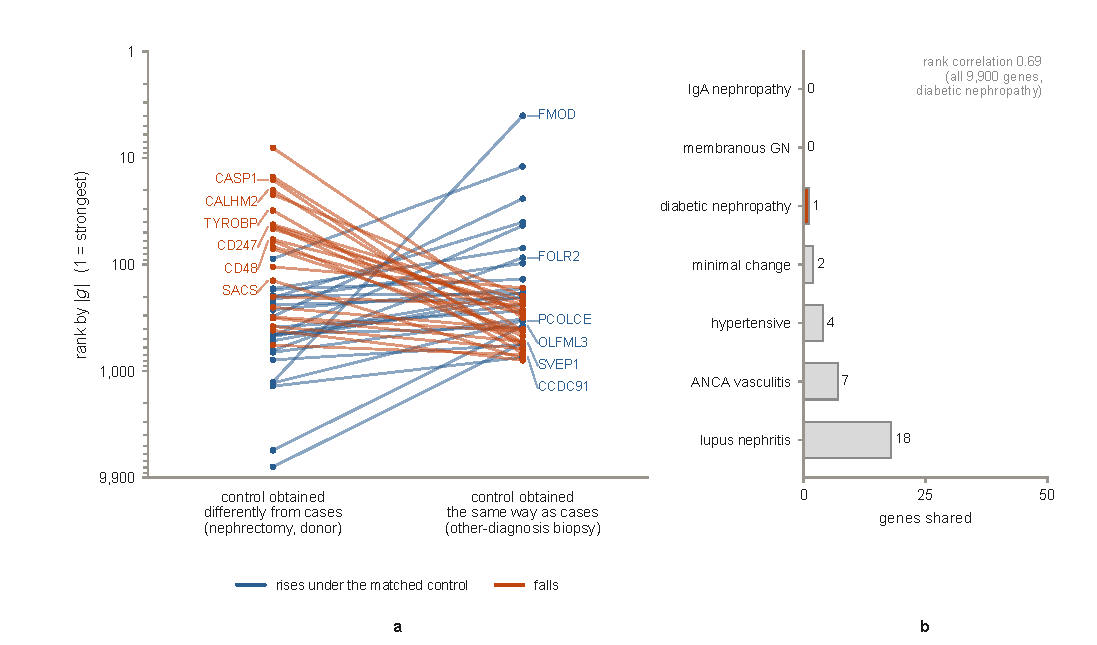
\includegraphics[width=\textwidth]{Fig4}
\caption{\textbf{Changing the control-group definition rebuilds the top of the ranking.} \textbf{a} Each line is one gene, drawn between its rank by $|g|$ when diabetic nephropathy cases are compared with non-biopsy controls (left) and with biopsies of other diagnoses (right); blue rises, orange falls. \textbf{b} Genes shared by the two top-50 lists, over all 9,900 genes, for each of the seven ERCB biopsy diagnoses. This is the same case set against two control groups, not a within-patient pairing.}\label{fig:reordering}
\end{figure*}

\subsection{Both mechanisms outside kidney: predictions fixed before the data}\label{sec:xtissue}

\textbf{Verdict instability (P1).} In liver the difference in cross-fold agreement between
stability selection and the connectivity comparator ranged from $-0.008$ to $+0.174$ across the ten
three-cohort subsets, crossing zero in one of the ten subsets tested and narrowly, while the
external AUROC difference stayed positive in all ten (Table~\ref{tab:xtissue}). That one reversal
is small, so we asked whether it is an artefact of the resampling seed. Repeating the ten
three-cohort comparisons under five bootstrap seeds reproduced it in the same subset
(GSE89632 $+$ GSE48452 $+$ GSE83452) every time, at $-0.017$ to $-0.008$, while the other nine
subsets stayed positive under all five seeds. The fifty runs are repeated computations on one
dataset rather than fifty independent tests, so this supports robustness to computational
randomness and says nothing about patient-sample uncertainty. P1 therefore holds in liver with
that scope: a small reversal, repeatable, in one configuration of ten. In colon it never crossed zero ($+0.006$ to
$+0.192$), and the prediction failed there. Post hoc, the tissues differed most in how far their
cohorts agree about the disease: the median pairwise correlation of gene-wise effect sizes was 0.66
in colon against 0.22 in kidney and 0.15 in liver. Subsampling colon cohorts to kidney sample
sizes produced only rare, small reversals: with each colon cohort subsampled to kidney case and
control counts, concordance stayed between 0.60 and 0.65 in five replicates, and the difference
crossed zero in two of them by at most 0.013 (Figure~\ref{fig:xtissue}c). Sign changes were
therefore associated with cohorts that disagree about the disease signal; concordance can be
computed before any method is run. Three tissues cannot establish it as a necessary condition.

\textbf{The module at the cohort level (P2).} Where cases were biopsies and controls surgical or
donor tissue, the score was lower in cases in 9 of 10 cohorts across kidney and liver, with liver
GSE89632 at $g = -4.60$ [$-6.11$, $-3.82$] (Figure~\ref{fig:xtissue}a; Supplementary Figure~S5). The prediction nonetheless
failed, because matched cohorts were not near zero: in colon the score was higher in inflamed
cases in 9 of 10 cohorts ($+0.51$ to $+3.43$). The module also responds to active inflammation.
Adjusting for the inflammation score shrank the colon effect by a median of 49\% and left every
biopsy-versus-surgical cohort negative, all ten after adjustment against nine before (median
standardised coefficient $-0.94$ before and $-1.14$ after; Mann--Whitney $p = 1.6 \times 10^{-4}$
against matched cohorts). The kidney attribution survives, and the one kidney cohort with a
positive raw effect turns negative once inflammation is accounted for.

\textbf{Reproducibility of the module (P3).} On each tissue's five core cohorts, the uncorrected
stability top 50 held a mean of 8.0 immediate-early genes in kidney, 0.6 in liver and 0.0 in colon,
and residualisation removed 7.2 of them in kidney (Figure~\ref{fig:xtissue}b). Liver carries the
largest procurement effects in this study, but only two of its five core cohorts are asymmetric;
colon shares a direction of effect, but there the module is one inflammation-responsive set among
stronger ones. Relaxing the liver expression filter raised module coverage from 11 to 15 genes and
left the count at 0.6. Post hoc, control substitution within liver GSE48452 moved the module effect
in the expected direction but with overlapping intervals, and is recorded as unresolved
(Supplementary Note~S10).

\begin{table*}[!t]
\caption{Predictions fixed before the liver and colon data were read, with the kidney reference computed by the same code}\label{tab:xtissue}
\tabcolsep=0pt
\begin{tabular*}{\textwidth}{@{\extracolsep\fill}>{\raggedright\arraybackslash}p{58mm}>{\raggedright\arraybackslash}p{29mm}>{\raggedright\arraybackslash}p{29mm}>{\raggedright\arraybackslash}p{29mm}>{\raggedright\arraybackslash}p{25mm}@{\extracolsep\fill}}
\toprule
Prediction & Kidney, DKD & Liver, MASH & Colon, UC & Verdict \\
\midrule
P1. The three-cohort RBS $-$ connectivity difference in cross-fold agreement spans zero & $-0.106$ to $+0.170$ (1 of 10 negative) & $-0.008$ to $+0.174$ (1 of 10) & $+0.006$ to $+0.192$ (0 of 10) & held in liver, failed in colon \\
\quad and the external AUROC difference changes sign in fewer subsets & $-0.027$ to $+0.153$ (2 of 10) & $+0.040$ to $+0.377$ (0 of 10) & $-0.005$ to $+0.067$ (1 of 10) & \\
P2. $|g_{\text{IEG}}| < 0.5$ in procurement-matched cohorts; negative, and larger than in every matched cohort, where cases are biopsies and controls surgical & 7 asymmetric, 6 negative & 3 asymmetric, all negative; 3 of 4 matched below 0.5 & 10 matched, 1 below 0.5, 9 positive & failed in both \\
P3. Immediate-early genes in the uncorrected stability top 50: kidney $>$ liver $>$ colon, colon at most 1; correction reduces the count substantially only in kidney & 8.0 (7.2 removed) & 0.6 (0.6 removed) & 0.0 & held \\
\botrule
\end{tabular*}
\begin{tablenotes}%
\item Wording abbreviated from the locally fixed prediction file (Supplementary File~7). The single negative liver subset recurs under five bootstrap seeds ($-0.017$ to $-0.008$), and the other nine stay positive in all five. Kidney values are a reference, not part of any prediction. By the same per-subset count the second clause of P1 would not hold in kidney either (2 AUROC sign changes against 1); the predictive verdict rests on the mean advantage per subset size, positive at every size in all three tissues. The kidney P3 count is a fold mean at the sweep's inner bootstrap size and so differs from the 10 of the headline run.
\end{tablenotes}
\end{table*}

\begin{figure*}[!t]
\centering
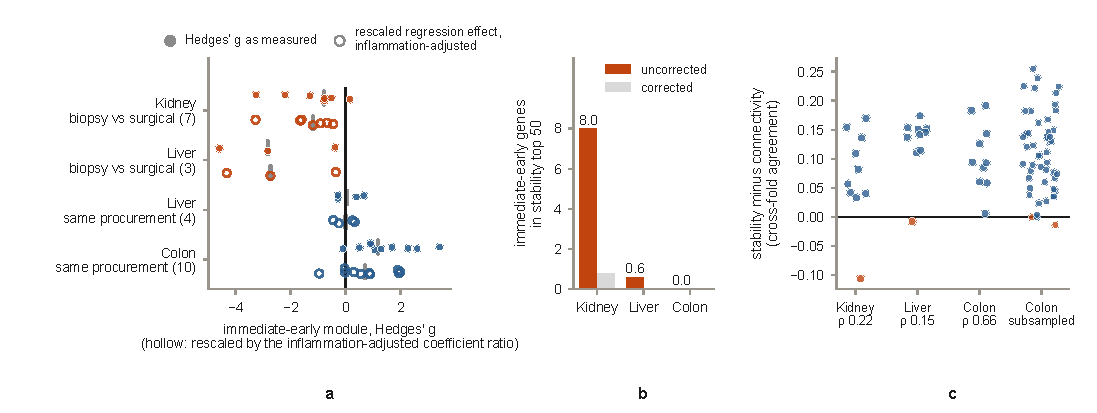
\includegraphics[width=\textwidth]{Fig5}
\caption{\textbf{Outside kidney, the immediate-early module follows procurement where it is asymmetric and inflammation where it is not, and reaches the most reproducible genes mainly in kidney.} \textbf{a} Hedges' $g$ of the handling score, case minus control, one point per cohort, grouped by tissue and by whether cases and controls were procured differently (biopsy vs surgical) or identically (same procurement); cohort counts in brackets. Filled points are $g$ as measured. Hollow points are not a second $g$: they are that $g$ multiplied by the ratio of the adjusted to the unadjusted standardised case coefficient from the inflammation regression, which carries the adjustment onto the same axis. The two coefficients themselves, on their own scale, are in Supplementary File~7 and their medians are quoted in the text. Bars mark group medians. Per-cohort values with accession labels and bootstrap intervals are in Supplementary Figure~S5. \textbf{b} Mean immediate-early genes in the stability top 50 over LODO folds on each tissue's five core cohorts, uncorrected and after residualising on the handling score. \textbf{c} Stability selection minus the connectivity comparator in cross-fold agreement for every three-cohort subset; orange points are reversed verdicts. $\rho$ is the median pairwise Spearman correlation of gene-wise effect sizes. The rightmost column repeats colon subsampled to kidney sizes. The inflammation adjustment, concordance and subsampling are post hoc. Custom co-expression hub comparator; not the reference WGCNA implementation.}\label{fig:xtissue}
\end{figure*}

\subsection{What the audit changes in a candidate list}\label{sec:candidates}

The last step of the protocol asks what the correction does to the output it is meant to protect.
Run with and without the handling-score correction, the pipeline returned 30 specificity-gated
candidates each time, sharing only 14. The corrected list moved towards established biology
(20 of 30 genes already proposed as DKD markers against 13 of 30), and the cell requiring a gene
to be both strong in the data and absent from the literature was empty before and after the
correction. Two candidates without prior DKD literature were removed by three independent tests,
and protein-level corroboration in two patient-independent datasets was positive but wide and
partly non-independent; Supplementary Note~S7 reports it with the qualifications. We therefore
report no novel biomarker, and read the value of the correction as diagnostic rather than
generative: it tells a reader that a list assembled without it is substantially a different list,
and that the difference does not run towards novelty.

%%=============================================================%%
\section{Discussion}\label{sec:discussion}
%%=============================================================%%

Cross-cohort consistency is a proxy for validity only when cohorts differ in the ways that matter.
In public DKD transcriptomics they do not: every discovery contrast compares biopsies with surgical tissue, so
the strongest shared signal is associated with procurement. This is a batch effect in the sense of Leek et al.\
\cite{leek2010}, aggravated by being confounded with the outcome by design. More cohorts of the
same design make such a confounder look more reproducible, not less. Applying the protocol to two
further tissues turned this into a conditional statement: the confounder appeared wherever
procurement was asymmetric, and was most prominent among the most reproducible genes where every
cohort shared that asymmetry.

The instability of benchmark verdicts has a broader reach. That rankings shift with benchmark
composition is not new \cite{boulesteix2013,jelizarow2010,ullmann2023,weber2019,norel2011}; what
these data add is its magnitude in a setting where reporting a single configuration is the norm,
the observation that reproducibility flips sign while the mean external AUROC advantage does not,
and an association: the flips went with cohorts that disagree about the disease signal, and in the
one tissue whose cohorts agreed closely, reversals stayed rare and small even after subsampling to
kidney cohort sizes. Three tissues are too few to treat concordance as a necessary condition or a
threshold, but it is cheap to compute before any selection is run, and a low value warns that a
single-configuration verdict is unlikely to transfer.

Three practical recommendations follow (Table~\ref{tab:checklist}). Report reproducibility and
validity as separate axes. Include a control obtained by the same procedure wherever one exists:
the 310 non-diabetic CKD biopsies in ERCB did more work than any algorithm in this study. And
report pre-analytical variables in the SPREC \cite{betsou2010,lehmann2012} or BRISQ
\cite{moore2011} format; had ischaemia time been recorded in any DKD cohort, the confounder would
be a covariate rather than an inference. The handling score is also computable per sample without
labels and can flag heterogeneous batches, but the cross-tissue test qualifies both that use and
the correction built on it. Because the module rises with active inflammation, residualising on
it in an inflamed tissue would remove disease biology with the artefact. In kidney the risk is
bounded, since adjusting for inflammation made the biopsy-versus-surgical effect larger, but it is
why we regard the score-based correction as tissue-conditional, and a control obtained by the
same procedure as the design alternative to prefer where clinically defensible and available.

\subsection{Limitations}\label{sec:limitations}

The empirical comparisons cover a limited set of established selection strategies,
including a custom co-expression hub comparator, rather than an exhaustive benchmark of
contemporary methods. The reversals recur under seven classical inner selectors and when the custom comparator is
replaced by the WGCNA package (Table~\ref{tab:selectors}), so they are not an artefact of the
reimplementation; the exclusion of the immediate-early module, by contrast, held for the
reimplementation and its 32 variants but not for the package on every fold, and appears to depend
on module detection rather than to be a property of connectivity criteria as a class. The magnitudes
reported apply to the implementations and cohort configurations examined here and should not be
generalised to entire method families. The audit procedure can be applied to additional selectors, but their sensitivity
to cohort composition remains to be evaluated.

The confounder-matched evidence in kidney rests on ERCB and KPMP, and GSE104948 contributed both to
discovery and to the specificity gate; re-deriving the candidates without it kept 17 of the 30 and
left the external replication intact (Supplementary Note~S8). The five discovery cohorts are few
for LODO-based claims, and the composition analysis quantifies rather than removes that
limitation. The simulation is deliberately simple. Outside kidney, only three liver cohorts had
asymmetric procurement, one with a mixed case arm; procurement was coded from series text and
publications rather than recorded handling; and the explanations offered for the two failed
predictions, inflammation and effect concordance, were examined only post hoc. The central claim
rests on single-modality transcriptomics: the proteomic and germline analyses corroborate or bound
it, and no public resource carries a multi-layer design complete enough to form a
diabetic-versus-control contrast in the same participants (Supplementary Note~S8).

%%=============================================================%%
\section{Conclusion}\label{sec:conclusion}
%%=============================================================%%

A difference in reproducibility between selection methods should be assessed together with its
cohort-composition sensitivity before it is generalised: in these data the verdict changed sign
across admissible subsets of the same cohorts, and the range mattered most where cohorts disagreed
about effects. The most reproducible signal in such a
comparison can be a pre-analytical confounder shared by design. Removing it changes which genes are
reported, only 14 of 30 candidates surviving, but does not produce a defensible novel candidate:
its value is diagnostic rather than generative. The checklist in Table~\ref{tab:checklist} and the
released code allow each check to be applied to other diseases before a candidate set is carried
forward.

%%=============================================================%%
\section{Supplementary data}
%%=============================================================%%

Supplementary data are available online at \textit{Briefings in Bioinformatics}. Supplementary
Notes S1--S10 extend the methods and results; Supplementary Files 1--7 contain the comparator
validation, the cohort audit, harmonisation and candidate tables, per-diagnosis results, the
full candidate evidence matrix, the proteomic cohort records, and the cross-tissue test with the
predictions as they were hash-fixed.

\section{Conflicts of interest}

The authors declare that they have no competing interests.

\section{Funding}

This research was supported by the National Research Foundation of Korea (NRF) grant funded by the
Korean government (MSIT) (No. RS-2026-25524613); by an internal research grant of the Electronics
and Telecommunications Research Institute (ETRI) (No. 25YT1400); and by the Culture, Sports and
Tourism R\&D Program through the Korea Creative Content Agency grant funded by the Ministry of
Culture, Sports and Tourism in 2024 (No. RS-2024-00398310).

\section{Data availability}

All transcriptome cohorts are available from GEO under accessions GSE30528, GSE30529, GSE96804,
GSE104948, GSE104954, GSE142025, GSE294519, GSE162830, GSE175759, GSE142153, GSE1009, GSE111154,
GSE20602 and GSE5406 (kidney and heart); GSE89632, GSE48452, GSE162694, GSE126848, GSE83452,
GSE66676, GSE63067 and GSE24807 (liver); and GSE75214, GSE87466, GSE179285, GSE11223, GSE47908,
GSE38713, GSE53306, GSE16879, GSE48958 and GSE13367 (colon). Single-nucleus data are available from
the KPMP Atlas (\url{https://atlas.kpmp.org/}). The protein datasets are Mendeley Data 83k89shdx5
and PRIDE PXD041884, the germline association study is GWAS Catalog GCST90179152, and the plasma
metabolome is Metabolomics Workbench ST003255. The harmonised matrices, frozen gene space,
%% BEGIN BIBAVAIL
phenotype tables with procurement annotation and the cohort audit database are deposited at
\url{https://doi.org/10.5281/zenodo.23051697}, and all code is available at
\url{https://github.com/kdh6126/dkd-cross-cohort-audit}.
%% END BIBAVAIL

\section{Author contributions statement}

D.K. conceived the study, designed the methodology, implemented the pipeline, curated the data,
performed the analyses and validation, produced the figures and wrote the manuscript. M.B., J.P.,
H.L. and H.J.L. contributed to the methodology and data curation and reviewed the manuscript.
S.L. acquired funding, administered the project and supervised the study. All authors reviewed
and approved the final manuscript.

\section{Acknowledgments}

The results reported here are in whole or in part based upon data generated by the Kidney
Precision Medicine Project (\url{https://www.kpmp.org}), accessed August 24, 2026. The KPMP study is
supported by the National Institute of Diabetes and Digestive and Kidney Diseases. We thank the
patient participants who consented to kidney biopsy for research, the European Renal cDNA Bank
consortium, and the investigators who deposited the public datasets analysed here.

\bibliographystyle{bib-vancouver}
\bibliography{dkd-references}

%% AUTHORS: BiB asks for a short description of each author. Title, affiliation and email only,
%% as requested. Emails were supplied by the authors on 2026-09-29.
\begin{biography}{}{\author{Dohun Kim} is a senior researcher at the Autonomous Intelligence DX Research Section, Electronics and Telecommunications Research Institute, Daejeon, Republic of Korea, and the corresponding author. Email: dohun@etri.re.kr.}
\end{biography}
\begin{biography}{}{\author{Minho Bae} is a senior researcher at the Autonomous Intelligence DX Research Section, Electronics and Telecommunications Research Institute, Daejeon, Republic of Korea. Email: minkkang@etri.re.kr.}
\end{biography}
\begin{biography}{}{\author{Jinho Park} is a senior researcher at the Autonomous Intelligence DX Research Section, Electronics and Telecommunications Research Institute, Daejeon, Republic of Korea. Email: jinho.park@etri.re.kr.}
\end{biography}
\begin{biography}{}{\author{Hayoung Lee} is a researcher at the Autonomous Intelligence DX Research Section, Electronics and Telecommunications Research Institute, Daejeon, Republic of Korea. Email: underzero11@etri.re.kr.}
\end{biography}
\begin{biography}{}{\author{Hyeokjin Lim} is a senior researcher at the Autonomous Intelligence DX Research Section, Electronics and Telecommunications Research Institute, Daejeon, Republic of Korea. Email: hyeokjin.lim@etri.re.kr.}
\end{biography}
\begin{biography}{}{\author{Seonghee Lee} is a principal researcher at the Autonomous Intelligence DX Research Section, Electronics and Telecommunications Research Institute, Daejeon, Republic of Korea. Email: slee0003@etri.re.kr.}
\end{biography}

\end{document}
